\documentclass[12pt]{article}
\usepackage[T1,LGR,T2A]{fontenc}
\usepackage[utf8]{inputenc}
\usepackage[greek,russian,english]{babel}
\usepackage{mathpazo}
\renewcommand{\familydefault}{\sfdefault}
\usepackage[landscape,a4paper]{geometry}
\geometry{verbose,tmargin=0cm,bmargin=0cm,lmargin=3cm,rmargin=3cm}
\usepackage{fancybox}
\usepackage{calc}
\usepackage{multicol}
\usepackage{graphicx}
\usepackage{url}
\usepackage{eso-pic}
\usepackage{textcomp}
\usepackage{paratype}
\usepackage{tgpagella}


\DeclareFontFamilySubstitution{T2A}{\rmdefault}{PTSerif-TLF}
\DeclareFontFamilySubstitution{LGR}{\rmdefault}{udidot}

\definecolor{myorange}{RGB}{226, 83, 48}

\newcommand\BackgroundPic{%
\put(0,0){%
\parbox[b][\paperheight]{\paperwidth}{%
\vfill
\centering
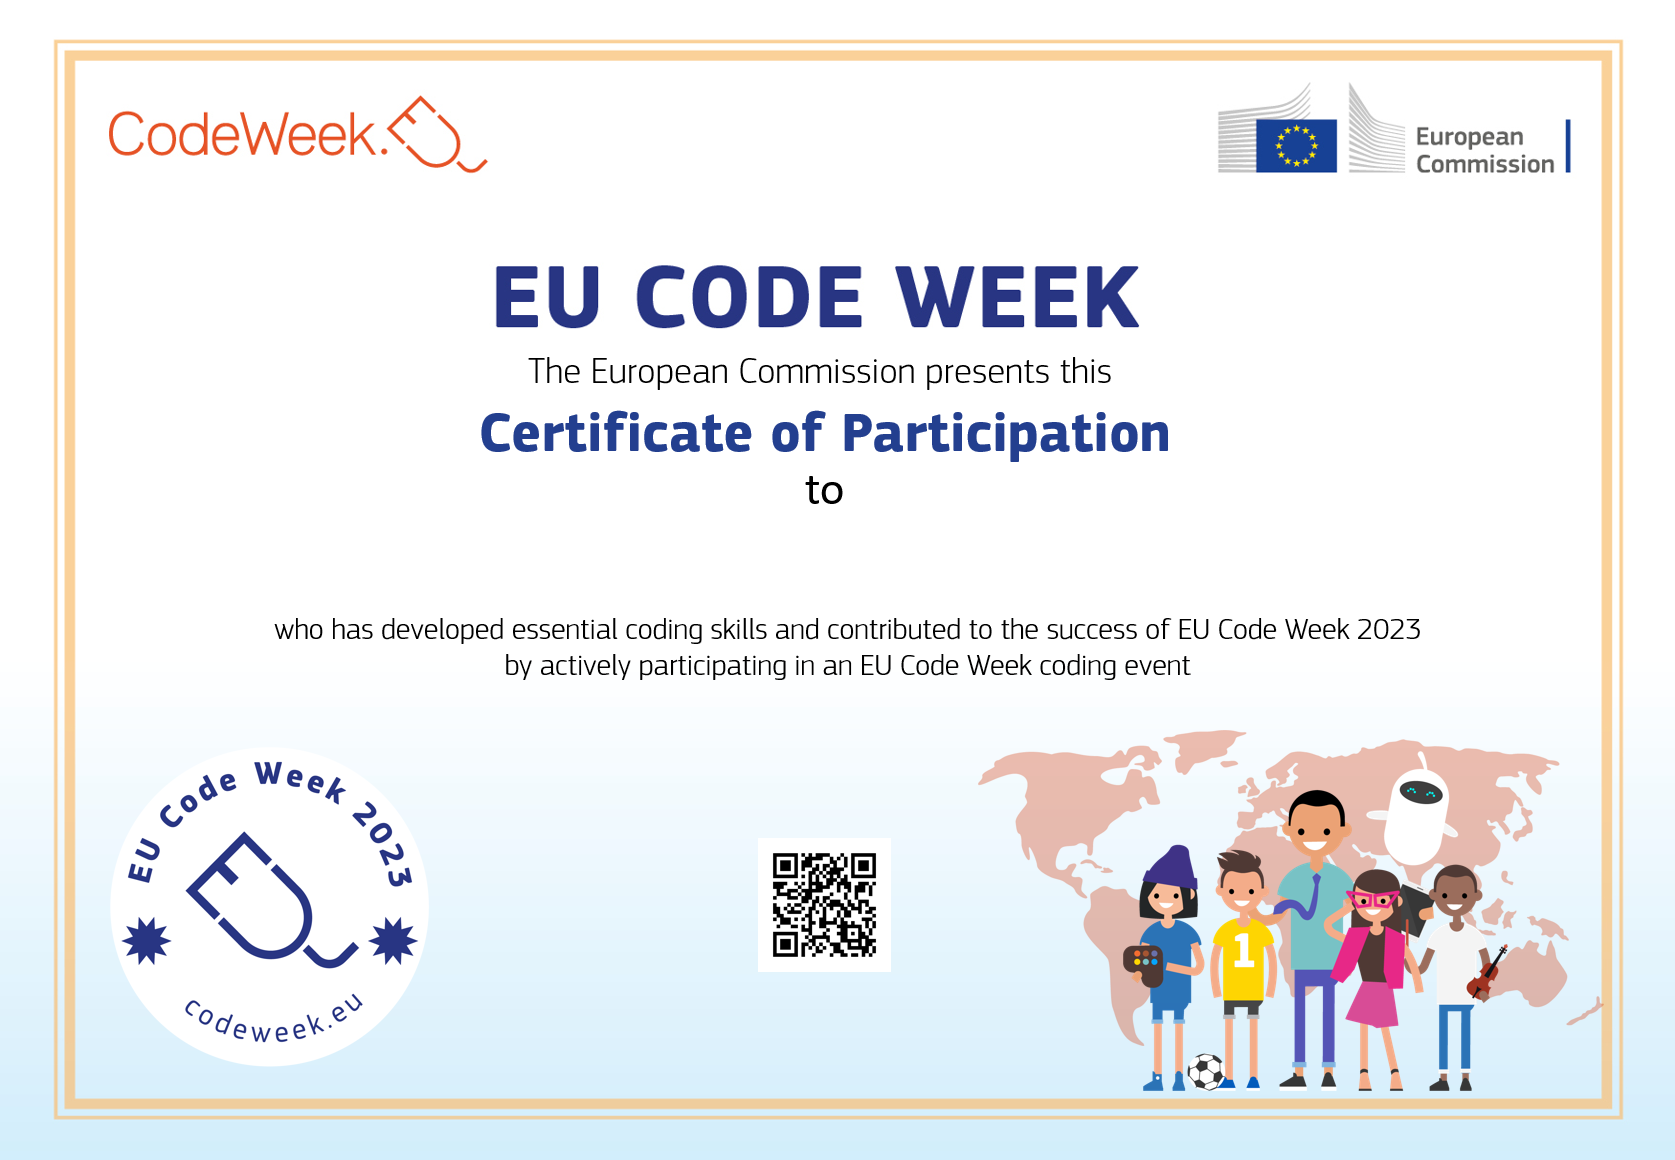
\includegraphics[width=\paperwidth,height=\paperheight,%
keepaspectratio]{images/participation-certificate-2024.png}%
\vfill
}}}

\begin{document}
\AddToShipoutPicture{\BackgroundPic}
~
\vspace{2.2cm}
~
\begin{center}

\vspace{5.9cm}

{\centering\fontsize{36}{48}\selectfont
\begin{otherlanguage*}{<CERTIFICATE_HOLDER_NAME_LANG>}
\textcolor{myorange}{<CERTIFICATE_HOLDER_NAME>}
\end{otherlanguage*}
\par}

\begin{table}[h]
\footnotesize

\begin{center}
\fontsize{24}{36}\selectfont
\vspace{1.6cm}
\begin{otherlanguage*}{<EVENT_NAME_LANG>}
\textcolor{myorange}{<EVENT_NAME>}
\end{otherlanguage*}
\end{center}
\end{table}

\end{center}
\vspace{2.2cm}
\begin{center}
\hspace{-0.5cm}
\begin{otherlanguage*}{<EVENT_DATE_LANG>}
\textcolor{black}{<EVENT_DATE>}
\end{otherlanguage*}
%\end{tabular}

\end{center}
\end{document}